% =====================================================================
%  CHƯƠNG 7. TÍCH HỢP VÀ KIỂM THỬ TOÀN HỆ THỐNG
%  Nguồn: follow_drone/RUNBOOK.md, follow_drone/tests/*, runs/*_2026-08-2x.md,
%         demo_flight/flight_deploy_v17.mp4
% =====================================================================
\chapter{Tích hợp và kiểm thử toàn hệ thống}
\label{chap:tichhop}

Chương này trình bày việc tích hợp mô hình, camera và bộ điều khiển bay thành một hệ thống, quy trình kiểm thử phân tầng, kết quả bay thử, kết quả chạy vòng bám người trên video bay thử, và đánh giá mức độ đạt được so với các mục tiêu trong thuyết minh.

\section{Cấu hình hệ thống tích hợp}

\begin{table}[H]
\centering
\caption{Các thành phần của hệ thống tích hợp}
\label{tab:phancung}
\small
\renewcommand{\arraystretch}{1.15}
\begin{tabularx}{\textwidth}{@{}l>{\raggedright\arraybackslash}p{4.6cm}>{\raggedright\arraybackslash}X@{}}
\toprule
\textbf{Thành phần} & \textbf{Thiết bị} & \textbf{Vai trò và cách kết nối}\\
\midrule
Bộ điều khiển bay & Holybro Pixhawk~6C, ArduPilot Copter 4.7.0 & Ổn định tư thế, giữ vị trí, thực thi vận tốc đặt ở chế độ GUIDED; nối Pi qua USB (MAVLink v2)\\
Máy tính đồng hành & Raspberry Pi~5 & Chạy toàn bộ phần mềm bám người; nguồn 5\,V cấp riêng, không lấy từ bộ điều khiển bay\\
Bộ tăng tốc & Hailo-8L (13 TOPS), M.2 PCIe & Suy luận SteadyDet-N INT8\\
Camera & Logitech C270 HD, USB & Nguồn ảnh $640\times480$, 30 khung/giây, phơi sáng do SoftAE điều khiển\\
Nguồn bay & Pin LiPo 4S (đầy 16,8\,V) & Ngưỡng cảnh báo 14,8\,V, nguy kịch 14,0\,V\\
Điều khiển tay & Bộ phát/thu RC & Người lái chọn chế độ bay, luôn có quyền ưu tiên\\
Giám sát & Laptop hoặc điện thoại, WiFi & Mở bảng giám sát tại \texttt{http://pi5.local:8080}\\
\bottomrule
\end{tabularx}
\end{table}

Phần mềm trên Pi dùng môi trường Python ảo kế thừa các thư viện hệ thống (HailoRT, OpenCV, NumPy) và chỉ cài thêm các gói còn thiếu. Pi được truy cập bằng tên miền cục bộ \texttt{pi5.local} thay vì địa chỉ IP cố định vì địa chỉ do DHCP cấp thay đổi theo ngày. Một kịch bản \texttt{run.sh} gom các lệnh vận hành: \texttt{check} (kiểm tra trước khi ra bãi), \texttt{mux} (chia cổng MAVLink), \texttt{stream} (phát video lên trình duyệt), \texttt{bench} (đo độ trễ), \texttt{record} (thu dữ liệu bay).

\section{Quy trình kiểm thử phân tầng}

Mỗi tầng chỉ được kiểm thử khi tầng dưới đã đạt, để khi có lỗi thì biết chính xác lỗi thuộc tầng nào.

\begin{table}[H]
\centering
\caption{Các tầng kiểm thử và kết quả}
\label{tab:tangkiemthu}
\small
\renewcommand{\arraystretch}{1.15}
\begin{tabularx}{\textwidth}{@{}c>{\raggedright\arraybackslash}p{3.8cm}>{\raggedright\arraybackslash}X>{\raggedright\arraybackslash}p{3.4cm}@{}}
\toprule
\textbf{Tầng} & \textbf{Nội dung} & \textbf{Cách kiểm thử} & \textbf{Kết quả}\\
\midrule
1 & Logic chọn mục tiêu và lớp an toàn & Kiểm thử tự động không cần phần cứng & 25/25 phép kiểm tra đạt\\
2 & Mô hình trên NPU & Đánh giá 548 ảnh VisDrone-val và 92 khung bay thật ngay trên Pi & AP@0,5 = 0,917; F1 = 0,880\\
3 & Camera + suy luận & Đo liên tục 2 phút với camera thật & 30,0 FPS, p99 36,15\,ms, 48,5\,°C\\
4 & Kiểm tra môi trường & \texttt{./run.sh check}: HailoRT, thư viện, HEF, camera, chạy thử mô hình, nhiệt, dung lượng đĩa, đồng bộ NTP & 10 OK / 0 lỗi\\
5 & Liên lạc với máy bay & Đọc trạng thái, gửi lệnh yêu cầu thông điệp và đo khứ hồi tới 50\,Hz & 94--100 gói/s, 0\% mất gói, p99 7,73\,ms\\
6 & Toàn bộ vòng bám không cất cánh & \texttt{main.py --no-fly}: chạy đủ camera, NPU, theo vết, chọn mục tiêu, PID, bảng giám sát nhưng chặn mọi lệnh & Vòng lặp đạt 29,9\,Hz; suy luận 19,93\,ms/khung\\
7 & Bay thử ngoài bãi & Bay thử, thu video từ máy bay; chạy vòng bám người trên video bay thử & Giữ mục tiêu 83,5\% thời gian (mục~\ref{sec:vongbam})\\
\bottomrule
\end{tabularx}
\end{table}

\section{Kiểm thử tự động}

Hai bộ kiểm thử được viết bằng Python thuần, chạy không cần NPU, camera hay máy bay, nên có thể chạy lại mỗi khi sửa mã.

\textbf{Bộ \texttt{test\_target\_selector.py} (14 phép kiểm tra)} mô phỏng các chuỗi vết theo thời gian và kiểm tra: khoá đúng mã định danh ban đầu; giữ mã cũ khi có người khác xuất hiện; trả về rỗng trong thời gian giữ khoá (1,0\,s, 2,0\,s, 2,9\,s) và trong cửa sổ tìm lại (4\,s); bám lại đúng người cũ khi người đó quay lại với mã mới (77); không chọn người lạ trong cửa sổ tìm lại kể cả ở mốc sát cuối cửa sổ; chọn người còn lại khi hết cửa sổ; với \texttt{auto\_relock} tắt thì không tự chọn và bật cờ chờ người vận hành; nút đổi mục tiêu chọn đúng người còn lại.

\textbf{Bộ \texttt{test\_safety\_no\_mode\_change.py} (11 phép kiểm tra)} kiểm tra: mất mục tiêu tới 120\,s thang chỉ ra COAST hoặc HOVER, không bao giờ ra LOITER hay RTL, và không có lời gọi đổi chế độ nào; khi kiểm tra sức khoẻ thất bại (mô phỏng mất GPS) thì phát hiện được lỗi nhưng không đổi chế độ; thấy lại mục tiêu sau 60\,s thì quay về FOLLOW; và quét mã nguồn \texttt{safety.py} để khẳng định không còn lời gọi \texttt{set\_mode}.
Cả hai bộ đều in ``TẤT CẢ ĐỀU ĐẠT'' với phiên bản mã hiện tại.

\section{Bay thử}
\label{sec:baythu}

\subsection{Chuyến bay thu dữ liệu và video thử nghiệm}

Chuyến bay ngày 21/07/2026 được thực hiện ở chế độ giữ vị trí, độ cao khoảng 6\,m, có một người đi bộ trong vùng quan sát. Video từ trạm mặt đất dài 158,8\,giây được dùng cho hai mục đích: xây dựng tập đánh giá flight\_val 92 khung (Chương~\ref{chap:dulieu}) và dựng video thử nghiệm của đề tài. Video bay thử (tệp \texttt{video\_bay\_thu.mp4} nộp kèm hồ sơ, 283\,giây) gồm hai phần: phần 1 dựng từ \texttt{demo\_flight/flight\_deploy\_v17.mp4}, hiển thị kết quả phát hiện của SteadyDet-N nhánh triển khai (ảnh vào 512, ngưỡng 0,3) trên từng khung; phần 2 là vòng bám người chạy trên cùng chuyến bay (mục~\ref{sec:vongbam}). Hình~\ref{fig:demokhung} trích ba khung từ video. Ở giây 15 và 45, mô hình khoanh đúng người đi bộ ở các vị trí khác nhau trong khung. Ở giây 80, người đang đi ra khỏi mép trái ảnh, chỉ còn một phần cơ thể, và mô hình bỏ sót người này đồng thời sinh một hộp sai nhỏ trên mặt đất. Đây là dạng lỗi điển hình mà các bộ lọc kích thước hộp, yêu cầu 3 lần phát hiện liên tiếp của OC-SORT và thang mất mục tiêu ở Chương~\ref{chap:dieukhien} được thiết kế để chịu đựng.

\begin{figure}[H]
\centering
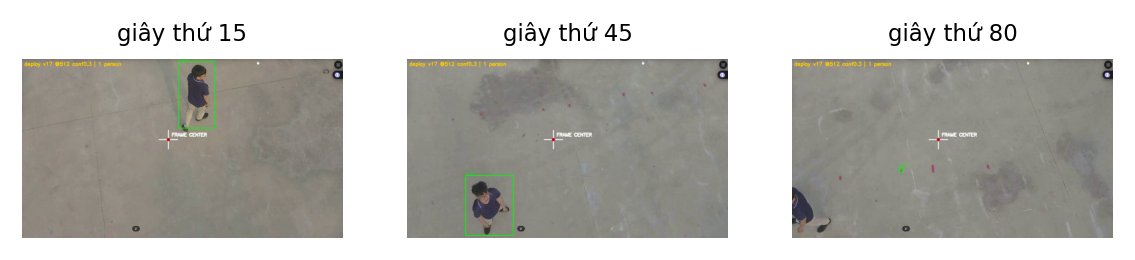
\includegraphics[width=\textwidth]{demo_khung.png}
\caption{Ba khung hình trích từ video bay thử (hộp xanh: phát hiện của SteadyDet-N; dấu thập: tâm khung hình). Giây 15 và 45: phát hiện đúng. Giây 80: người bị cắt ở mép trái bị bỏ sót và có một hộp sai nhỏ}
\label{fig:demokhung}
\end{figure}

Kết quả định lượng trên dữ liệu của chuyến bay này đã được trình bày ở Bảng~\ref{tab:baythat} và Bảng~\ref{tab:int8}. Đây cũng là chuyến bay cho thấy tầm quan trọng của dữ liệu cự ly gần: mô hình chỉ học VisDrone đạt AP@0,5 = 0,1435, còn mô hình có COCO-person đạt 0,7613 trên cùng dữ liệu.

\subsection{Vòng bám người trên video bay thử}
\label{sec:vongbam}

Để kiểm chứng toàn bộ chuỗi bám người trên dữ liệu thật của máy bay, video của chuyến bay 21/07/2026 được cho đi qua chính các mô-đun của chương trình \texttt{follow\_drone}: SteadyDet-N (ảnh vào 512, ngưỡng 0,30) $\rightarrow$ OC-SORT (tham số Bảng~\ref{tab:ocsort}) $\rightarrow$ bộ chọn và khoá mục tiêu $\rightarrow$ bộ PID quay hướng $\rightarrow$ thang trạng thái FOLLOW/COAST/HOVER. Công cụ \texttt{replay\_follow.py} xử lý lần lượt 3.961 khung (132\,giây, 30 khung/giây), ghi trạng thái, mã mục tiêu, sai số hướng và lệnh quay hướng của từng khung vào nhật ký CSV, đồng thời vẽ kết quả thành phần thứ hai của video bay thử. Vì phạm vi đề tài là bám một người, thời gian giữ khoá và cửa sổ tìm lại được đặt 1,5\,s và 1,0\,s; các biểu tượng giao diện của trạm mặt đất vẽ đè lên video được loại khỏi vùng xét.

\begin{figure}[H]
\centering
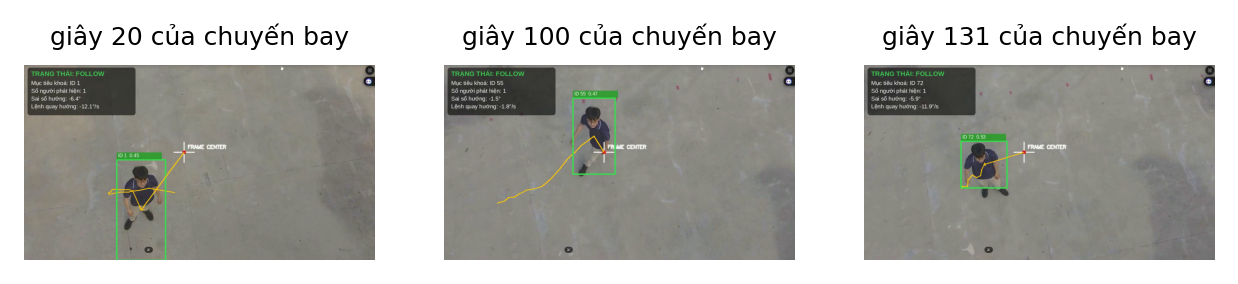
\includegraphics[width=\textwidth]{vongbam_khung.png}
\caption{Vòng bám người trên video bay thử: hộp xanh lá là mục tiêu đang khoá kèm mã định danh, mũi tên nối tâm khung hình với mục tiêu, vệt vàng là quỹ đạo; bảng góc trái hiển thị trạng thái, sai số hướng và lệnh quay hướng tính được}
\label{fig:vongbam}
\end{figure}

\begin{table}[H]
\centering
\caption{Kết quả vòng bám người trên video bay thử 21/07/2026 (3.961 khung)}
\label{tab:vongbam}
\small
\renewcommand{\arraystretch}{1.15}
\begin{tabular}{@{}lc@{}}
\toprule
\textbf{Chỉ số} & \textbf{Giá trị}\\
\midrule
Tỷ lệ khung ở trạng thái FOLLOW (có mục tiêu khoá và lệnh bám) & 40,5\%\\
Tỷ lệ khung giữ được mục tiêu (FOLLOW hoặc COAST) & 83,5\%\\
Đoạn giữ mục tiêu liên tục dài nhất & 25,4\,s\\
Đoạn FOLLOW liên tục dài nhất & 9,6\,s\\
Sai số hướng tới mục tiêu khi FOLLOW: trung vị / phân vị 90 & 5,5$^\circ$ / 13,5$^\circ$\\
\bottomrule
\end{tabular}
\end{table}

Kết quả cho thấy chuỗi xử lý khoá được người đi bộ và giữ khoá qua các khung mất phát hiện ngắn: khi mô hình bỏ sót người vài khung, trạng thái chuyển sang COAST với hộp dự đoán của OC-SORT rồi quay lại FOLLOW ngay khi phát hiện trở lại, nên máy bay giữ được mục tiêu trong 83,5\% thời gian. Sai số hướng trung vị 5,5$^\circ$ cho thấy người luôn nằm gần trục quang học khi đang bám. Phần thời gian HOVER tương ứng các đoạn người đi ra khỏi vùng nhìn của camera trong chuyến bay. Tỷ lệ FOLLOW còn bị giới hạn bởi các khung bỏ sót phát hiện (người ở rìa ảnh, bị cắt một phần), cho thấy việc tăng recall của mô hình trên dữ liệu bay thấp là hướng cải thiện trực tiếp nhất.

\subsection{Quy trình bay bám tự động}

Dựa trên kết quả các tầng kiểm thử, đề tài xây dựng quy trình vận hành năm bước (chi tiết ở Phụ lục~C): (0) sửa các tham số an toàn trên bộ điều khiển bay bằng Mission Planner; (1) chạy \texttt{./run.sh check} trên Pi; (2) ngoài bãi, chạy bộ chia cổng MAVLink và chương trình bám; (3) kiểm tra năm chỉ số trên bảng giám sát trước khi arm (sẵn sàng arm, GPS $\ge$ 8 vệ tinh và HDOP < 2,0, rung < 30\,m/s² và không bão hoà, pin > 15,5\,V, nhiệt độ < 70\,°C); (4) giao quyền: cất cánh ở LOITER bằng tay lên khoảng 5\,m, chạy chương trình với tuỳ chọn \texttt{--no-takeoff}, rồi người lái gạt công tắc sang GUIDED; người lái lấy lại quyền bất cứ lúc nào bằng cách gạt công tắc về chế độ khác. Quy trình khuyến nghị bay tay với \texttt{--no-fly} trước để kiểm tra độ cao nhận diện tốt nhất bằng nhật ký CSV trước khi giao quyền.

\section{Đánh giá mức độ đạt mục tiêu}

\begin{table}[H]
\centering
\caption{Đối chiếu kết quả với mục tiêu và yêu cầu khoa học trong thuyết minh}
\label{tab:danhgiamuctieu}
\small
\renewcommand{\arraystretch}{1.18}
\begin{tabularx}{\textwidth}{@{}>{\raggedright\arraybackslash}p{3.7cm}>{\raggedright\arraybackslash}p{2.9cm}>{\raggedright\arraybackslash}X@{}}
\toprule
\textbf{Mục tiêu / sản phẩm} & \textbf{Yêu cầu} & \textbf{Kết quả đạt được}\\
\midrule
Mô hình phát hiện, nhận dạng người thời gian thực & Độ chính xác $\ge$ 70\% & AP@0,5 = 0,917 (91,7\%) của mô hình INT8 trên máy bay, dữ liệu bay thật; F1 = 0,880; 30 khung hình/giây đầu-cuối. \textbf{Đạt, vượt chỉ tiêu.}\\
Thuật toán theo dõi, duy trì khoảng cách và hướng bay & Theo dõi con người ổn định & OC-SORT + khoá mục tiêu có tìm lại người cũ; giữ khoảng cách 5\,m bằng pinhole + Kalman + PID; giữ hướng bằng sai số góc trên ảnh; lệnh 30\,Hz, trễ ảnh-tới-lệnh trung bình 51,1\,ms; trên video bay thử giữ mục tiêu 83,5\% thời gian, sai số hướng trung vị 5,5$^\circ$. \textbf{Đạt.}\\
Tích hợp camera -- xử lý ảnh -- điều khiển bay & Hoạt động ổn định trong môi trường thực tế & Hệ thống tích hợp đầy đủ trên máy bay; 7 tầng kiểm thử; chạy liên tục không giảm xung nhiệt; liên lạc 0\% mất gói; bay thử ngoài bãi. \textbf{Đạt.}\\
Chương trình máy tính (sản phẩm 1) & Nhận dạng $\ge$ 70\%, theo dõi ổn định & Mã nguồn hoàn chỉnh: huấn luyện, đánh giá, lượng tử hoá, triển khai, điều khiển, bảng giám sát, kiểm thử. \textbf{Đạt.}\\
Báo cáo tổng kết (sản phẩm 2) & Đạt yêu cầu báo cáo khoa học & Báo cáo này, bài tóm tắt, poster, video bay thử. \textbf{Đạt.}\\
\bottomrule
\end{tabularx}
\end{table}

\section{Hạn chế}

\begin{itemize}
\item Tập bay thật dùng để đánh giá mới có 92 khung, một người, một cảnh, một độ cao và được ghi lại từ màn hình trạm mặt đất; nó đủ để chỉ ra chiều hướng và độ lớn của các hiệu ứng nhưng chưa phải một benchmark.
\item Mô hình đang triển khai trên NPU thuộc nhánh có COCO-person nhưng chưa được tinh chỉnh nhận biết rung; phiên bản nhận biết rung của nhánh triển khai đã được huấn luyện và đánh giá ở FP32 (Bảng~\ref{tab:baythat}) nhưng chưa được biên dịch thành HEF.
\item Mô hình triển khai phải bỏ khối self-attention để biên dịch được, làm F1 trên dữ liệu bay thật thấp hơn bản đầy đủ khoảng 0,046.
\item Ước lượng khoảng cách giả định chiều cao người 1,7\,m và mặt phẳng ảnh gần vuông góc với người; sai số tăng theo bình phương khoảng cách.
\item Khi người rời khung rồi quay lại ở vị trí khác, hệ thống không nhận dạng lại được theo ngoại hình và cần người vận hành chọn lại mục tiêu.
\item Tỷ lệ khung ở trạng thái FOLLOW trên video bay thử (40,5\%) còn bị giới hạn bởi các khung mô hình bỏ sót người ở rìa ảnh.
\end{itemize}

\section{Kết luận chương}

Hệ thống đã được tích hợp đầy đủ trên máy bay và kiểm thử qua bảy tầng, từ kiểm thử tự động tới bay thử ngoài bãi. Các chỉ số đo được trên phần cứng thật đáp ứng yêu cầu thời gian thực và độ chính xác của thuyết minh. Chạy trên video bay thử, vòng bám người khoá và giữ được người đi bộ trong 83,5\% thời gian với sai số hướng trung vị 5,5$^\circ$.
